\section{Foundations}									\label{sec:foundations}

\subsection{Grids}											\label{sec:grids}

A grid partitions (tessellates) some space into a discrete number of cells. In meteorology, the three-dimensional space of the atmosphere is subdivided by a grid to facilitate finding numerical solutions to equations governing the weather. Each cell may contain one or multiple values (\emph{fields}) such as the temperature or humidity at a location.

One kind of grid is the \emph{regular grid}. In this type of \emph{structured grid}, each cell is of uniform size and has a a fixed amount of six direct neighbors (top, bottom, left, right, front and back). Real-life objects that have the structure of a regular grid are checkerboards (two dimensions) or a Rubik's cube (three dimensions). Because of its regularity, storing such a grid in memory is straightforward.

In certain use cases, the use of \emph{unstructured grids} is beneficial to the requirements of the application at hand. In contrast to regular grids, cells need not be of equal size in unstructured grids and may have a varying number of neighbors. This means that a location of a cell's neighbor in memory does no longer follow a regular structure. Because neighbor's locations are no longer inherently clear, an unstructured grid requires an neighborship table to describe its structure. Accessing a neighbor requires an indirect memory lookup in order to determine its location in memory.

This thesis is concerned with the performance implications that porting a stencil computation from a regular to a unstructured grid entails. It compares the cost indirect addressing imposes upon several different widely-used stencils.

While an unstructured grid theoretically supports arbitrary neighborship relations, for this thesis, we restrict irregularities to the X-Y-plane and assume even unstructured grids are regular (i.e. always have at most two neighbors) in the Z-dimension. This is a common use case in meteorology. In practice, such as in so-called \emph{icosahedral grids}, most of the neighborships in the X-Y-plane will also most often have some structure to it. We make use of these regularities in the optimizations described in section \ref{sec:grid-implementations} and \ref{sec:optimizations}.


\subsubsection{Coordinates and Indices}

In our implementations, cells in a grid are identified by \emph{coordinates}, which relate a cell to its real-world position and \emph{indices} which give the storage location of a cell in memory. 

Throughout the rest of this report we refer to the dimensions of a grid as the \emph{maximum number of elements} in each dimension, and denote it by the vector
$$d = \begin{pmatrix}d_x \\ d_y \\ d_z\end{pmatrix}.$$
A unique identifier for each cell on the grid is given by its coordinates, denoted in similar fashion by a vector
$$p = \begin{pmatrix}p_x \\ p_y \\ p_z\end{pmatrix}.$$
The coordinates correspond to a position in Euclidian space. Coordinates are chosen such that each integer coordinate maps \emph{uniquely} to at most one cell. The opposite (i.e. each cell having only one coordinate) is only true in regular grids. In the regular grid, direct neighbors (adjacent/face-touching cells) differ in only one coordinate by an amount of one. In unstructured grids, not every coordinate is necessarily assigned to any cell, and one cell may span multiple coordinates. Therefore, an unstructured cell's neighbor might have coordinates that differ by more than one.

As memory is one-dimensional, a mapping from the three-dimensional coordinates of a cell to its location in memory is required of a grid implementation. We call this location in memory the \emph{index} and denote it with the letter $i$. The mapping from three-dimensional coordinate space to the one-dimensional memory index defines the memory layout of the grid. In regular grids, this mapping is straightforward, while in unstructured grids it may be arbitrary. How regular and unstructured grids are laid-out in memory is detailed in section \ref{sec:grid-implementations} (Grid implementations).

\subsection{Stencils}									\label{sec:stencils}

Finding approximate numerical solutions to the governing equations of physical processes, as in meteorology, often entails performing certain unchanging calculations on every cell of a grid. The result of this process is again a grid of similar dimensions. For each cell, the calculated output value is dependent only on a bounded, small number of neighboring cells' values (\emph{neighborhood}). Such a computation is called \emph{stencil}. Simple stencils may require only the values of the current cell as well as directly adjacent (face-touching) neighbors in order to calculate the output value, while more complex ones could also depend on diagonal neighbors, neighbors-of-neighbors etc. Yet, some spatial locality is guaranteed. 

\paragraph{Halo} \ref{sec:halo} In stencil computations, special consideration needs to be given to the boundary cells of the grid. Cells at the boundary of a grid have fewer neighbors than inner cells. As such, the output value for a stencil depending on neigbhors is unclear for cells who do not have those neighbors. One way to address this issue is to execute the stencil only on the safe inner values of a grid, seperated from the boundary by a certain padding. The amount of padding used depends on the size of the neighborhood which a stencil requires for its computation. We call the set of cells residing in the padding around the boundaries of the grid \emph{halo}. Stencil implementations may include a branch instruction that prevents any computations if a cell lies in the halo. Alternatively, for ease of implementation and performance, it can be beneficial to store the halo seperately in memory.

\subsection{GPU Programming on the Nvidia CUDA Platform}

\emph{Graphics processing units} (GPUs) particularly lend themselves to stencil computations. In this section, we contrast the execution model of classical \emph{central processing units} (CPUs) with that of GPUs. We explain why stencil applications can profit from execution on the GPU and elaborate the fundamentals of the \emph{Nvidia CUDA} platform for execution on the GPU.

Most classical computer programs run sequentially on the CPU. Computations are performed step-by-step. Such a sequence of operations is called \emph{thread}. First CPUs were only capable of running one thread at a time. Even today, only a handful of threads, i.e. execution streams, can run truly in parallel on a CPU. Operating on large data sets on the CPU therefore still mostly involves repeated calculations within loops which handle one data point at a time.

Most performance optimizations in CPUs target \emph{latency}; caches, pipelining, branch prediction and similar techniques aim to reduce the time between issuing a command and storing its result. While CPUs have become much faster since their inception, the improvements to performance have recently slowed due to physical constraints.

Sustained demands for faster runtimes and more complex applications have thus forced rethinking of the sequential execution model. Many real-world applications on large data sets consist of largely unvarying computations on many datapoints. These applications often have few sequential dependencies. Applications in computer grpahics, for example, often entail highly monotone computations that are repeated for every pixel displayed on the screen. The resulting value of the pixel at one edge of the screen probably does not require knowing about the result of a pixel at the other end, but sequential execution still dictates one value being calculated before the other. This observation spurred the development of parallel architectures, such as in GPUs. GPUs overcome the performance limits of sequential computation by providing thousands of hardware units which are able to compute (run threads) independently from one another, at the same time.\cite[Chapter~2]{cuda-for-engineers} This increases the \emph{throughput} of those devices: While a \emph{low-latency} CPU reacts to an issued command fast, it provides only one result for one datapoint. Meanwhile, a \emph{high throughput} GPU might take a longer time to issue the command, but it calculates the results for several datapoints ``at once''.

CPUs therefore shine in scenarios where calculations are less straightforward and predictable, while GPUs are more useful whereever monotone computations on large data sets are performed. Another advantage of GPUs is \emph{scalability}: Because the performed parallel computations are completely independent, larger problem sizes can effectively be made more efficient simply by adding more parallel execution capabilities to the hardware, i.e. adding more processors. Despite the name, GPUs are today no longer just used for graphics processing.

The task of applying a stencil to a grid (sections \ref{sec:grids}, \ref{sec:stencils}) greatly benefits in terms of performance from execution on highly parallel architectures such as graphics processing units (\emph{GPUs}), as it can easily be parallelized by decomposing the problem domain. Each thread may be responsible for calculating the result of one cell or a small set of cells in the output grid. As data dependencies are limited to a local neighborhood, parallel threads can work on spatially separated data concurrently without risk of data races in most cases. Data races only occur if threads share some dependencies, i.e. when their neighborhood overlaps. In that case, each thread can re-compute its dependencies (called \emph{computation on-the-fly}) or threads may share their results by means of \emph{synchronization}.

In this thesis, we use the \emph{Nvidia CUDA} architecture to implement meteorological stencil computations on the \emph{Nvidia Tesla V100} GPU, and we assess their performance on different types of grids.

\subsubsection{SIMT Execution Model}

\emph{CUDA} employs a \emph{Single Instruction, Multiple Thread (SIMT)} execution model. This model can be compared to the \emph{Single Instruction, Multiple Data (SIMD)} model but makes writing programs more straight-forward to programmers experienced in sequential programming.\cite[Section~3.1]{ptx-isa} 

In a \emph{SIMD} model, instructions are ``wide'': They support input operands that are larger than single scalar values. Programmers explicitly issue these \emph{vector instructions} to perform a calculation on a set of values. In contrast, in the SIMT model used by \emph{CUDA}, programmers do not need to explicitly perform operations on multiple data points. Instead, code is written such that it operates on single scalar values. Many instances, i.e. \emph{threads}, of this code are run which differ only in a input \emph{thread index} they receive. In most applications, this input is used to determine which datapoint the thread opeates on. Upon execution, when the same operation is executed in many threads on consecutive data points, they are grouped together automatically to be executed in parallel in SIMD-like fashion.

\subsubsection{Software}

Code to be executed on the GPU is written in specially-anotated functions called \emph{kernels}. Kernels can be written as regular C code but are compiled by the distinct Nvidia compiler \emph{(nvcc)} to \emph{Parallel Thread Execution (PTX)} machine code which can be run on the GPU. Inside a kernel, a \emph{thread and block index} is made available. Using a special syntax recognized by \emph{nvcc}, kernels can be launched from the CPU onto the GPU (sometimes simply called \emph{device}, as opposed to \emph{host} which refers to the CPU). The \emph{CUDA} Application Programming Interface (API) provides a device synchronization routine, which is required to synchronize CPU and GPU after computation of the kernel on the GPU is completed. This enables relatively simple offloading of parallelizable workloads onto the GPU as a coprocessor while continuing to run the rest of the program asynchronously on the CPU. The \emph{CUDA} API furthermore provides routines for memory allocation on the device, memory prefetching (see \ref{sec:unified-memory} unified memory) and setting certain device parameters.

\begin{lstfloat}
\begin{lstlisting}[caption={Example showing kernel, its launch and CUDA API calls for allocating unified memory},captionpos=b,language=C]
// Kernel Definition. This function runs on the GPU.
__global__
void multiply(double fac, double *input, double *output) {
	int i = threadIdx.x + blockIdx.x*blockDim.x;
	output[i] = fac * input[i];
}

// Kernel Invocation. This function runs on the CPU.
int main(int argc, char **argv) {
	double *input, output;
	int N = 1024 * 1024;
	cudaMallocManaged(&input, N * sizeof(double));
	cudaMallocManaged(&output, N * sizeof(double));
	cudaMemset(input, 42.0, N * sizeof(double));
	multiply<<<N/256, 256>>>(3.0, input, output);
	cudaDeviceSynchronize();
	cudaFree(input);
	cudaFree(output;)
}
\end{lstlisting}
\end{lstfloat}

\subsubsection{Streaming Multiprocessors} \label{sec:hardware}

\emph{CUDA}-capable GPUs are structured as an array of so-called \emph{Streaming Multiprocessors (SMs)}. Each SM contains a multitutde of scalar processor cores. These cores include arithmetic, logic and floating point units (ALUs, FPUs) and perform the actual computations on the data points. Together, they are used to advance computation in a \emph{warp}. A warp is a set of (typically 32) threads that are executed concurrently on the same multiprocessor. In every cycle, each thread inside a warp uses one of the scalar cores to execute the same instruction (on different data), or it is turned off if a branch diverged previously. A warp of multiple threads at the same instruction pointer executing the same instruction is therefore similar to executing a SIMD instruction on multiple datapoints.

Each SM has its own scheduler and operates completely independently of the other SMs. If the threads inside a warp diverge (because of branching instructions), the different execution paths are executed sequentially on the SM. It is therefore paramount to performance that kernels are written in such a way that threads in the same warp follow the same execution path whenever possible. One way to achieve this is to ensure branch conditions involve only the thread index divided by 32 (i.e. the warp size), as this will be the same value for all threads inside a warp. 

SMs chose the threads to form a warp from a pool of threads called a \emph{block}. When one warp finishes executing or is stalled (e.g. because of a memory dependency), the next set of threads forming a warp in the block is chosen to be executed. All threads in a block execute on the same SM. Resources such as registers and shared memory are divided among all threads in a block. Threads in the same block can communicate with one another through shared memory. Using the \texttt{\_\_syncthreads()} command in a kernel synchronizes all threads in the same block.

When a kernel is launched, the programmer may specify how many threads should be part of the same block (\emph{block size}), and how many blocks there should be (\emph{grid size}). These parameters are called the \emph{launch configuration}. It is important to have more blocks than SMs, as otherwise some SMs will have no work to perform. Furthermore, if a synchronization instruction is used in the kernel, it is beneficial to have multiple blocks per SM, as to occupy the SM when one of the blocks is stalling because it is waiting for synchronization. The number of threads per block (block size) should be a multiple of 32 to ensure warps can be entirely filled with threads. \cite[Section~10]{cuda-best-practices}

\subsubsection{Memories} \label{sec:memories}

There are several types of memory address spaces available in kernel code. Figure \ref{fig:memory-hierarchy} shows these address spaces in the programming model on the left, and how they are implemented in hardware with caches in the Volta architecture on the right. 

\begin{figure}
	\makebox[\textwidth]{
	


\tikzset{every picture/.style={line width=0.75pt}} %set default line width to 0.75pt        

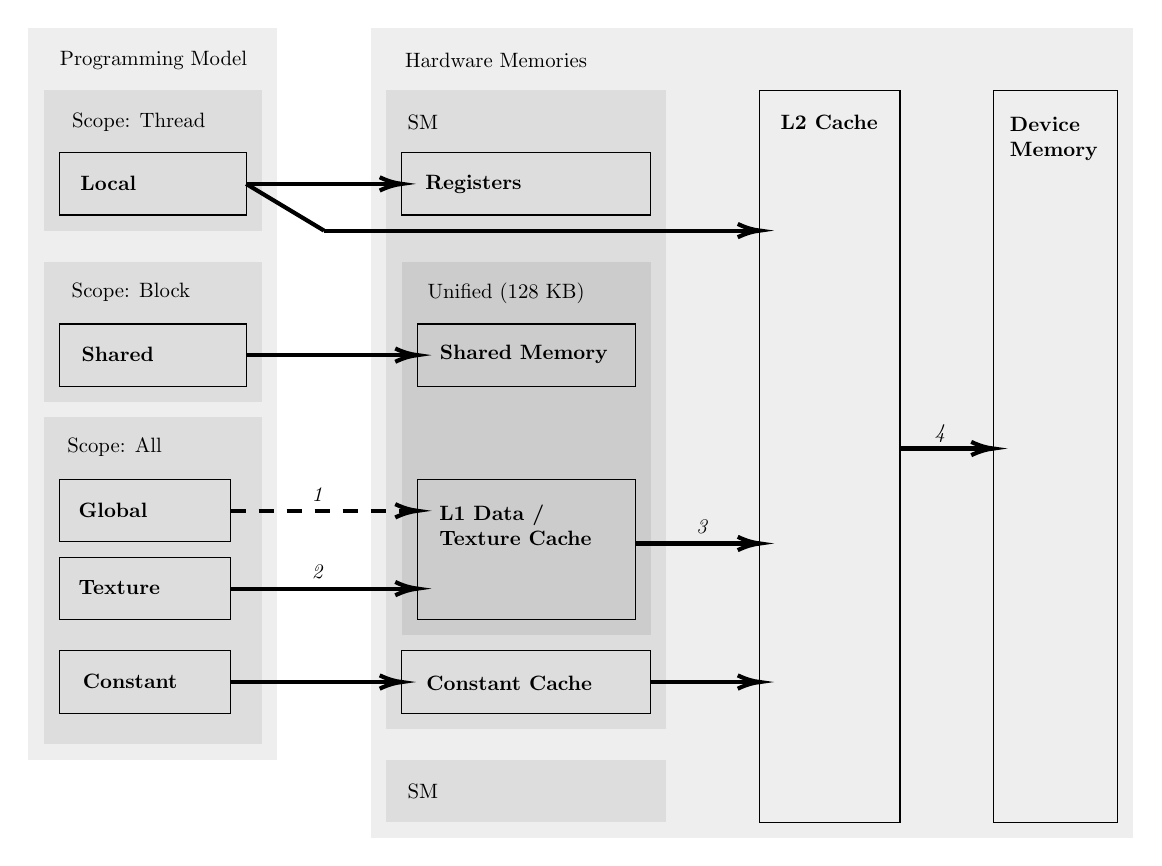
\begin{tikzpicture}[x=0.75pt,y=0.75pt,yscale=-0.75,xscale=0.75, every node/.style={scale=0.75}]
%uncomment if require: \path (0,574); %set diagram left start at 0, and has height of 574

%Shape: Rectangle [id:dp49466026838319044] 
\draw  [draw opacity=0][fill={rgb, 255:red, 238; green, 238; blue, 238 }  ,fill opacity=1 ] (10,10) -- (170,10) -- (170,480) -- (10,480) -- cycle ;
%Shape: Rectangle [id:dp28817003892392545] 
\draw  [draw opacity=0][fill={rgb, 255:red, 221; green, 221; blue, 221 }  ,fill opacity=1 ] (20,50) -- (160,50) -- (160,140) -- (20,140) -- cycle ;
%Shape: Rectangle [id:dp36092800198336605] 
\draw   (30,90) -- (150,90) -- (150,130) -- (30,130) -- cycle ;
%Shape: Rectangle [id:dp731633578877624] 
\draw  [draw opacity=0][fill={rgb, 255:red, 221; green, 221; blue, 221 }  ,fill opacity=1 ] (20,160) -- (160,160) -- (160,250) -- (20,250) -- cycle ;
%Shape: Rectangle [id:dp9265995086938097] 
\draw   (30,200) -- (150,200) -- (150,240) -- (30,240) -- cycle ;
%Shape: Rectangle [id:dp7383874820875151] 
\draw  [draw opacity=0][fill={rgb, 255:red, 221; green, 221; blue, 221 }  ,fill opacity=1 ] (20,260) -- (160,260) -- (160,470) -- (20,470) -- cycle ;
%Shape: Rectangle [id:dp3490802882861901] 
\draw   (30,300) -- (140,300) -- (140,340) -- (30,340) -- cycle ;
%Shape: Rectangle [id:dp7130701095363465] 
\draw   (30,410) -- (140,410) -- (140,450) -- (30,450) -- cycle ;
%Shape: Rectangle [id:dp4095820299975792] 
\draw   (30,350) -- (140,350) -- (140,390) -- (30,390) -- cycle ;
%Shape: Rectangle [id:dp6482924830961656] 
\draw  [draw opacity=0][fill={rgb, 255:red, 238; green, 238; blue, 238 }  ,fill opacity=1 ] (230,10) -- (720,10) -- (720,530) -- (230,530) -- cycle ;
%Shape: Rectangle [id:dp1781724326419385] 
\draw  [draw opacity=0][fill={rgb, 255:red, 221; green, 221; blue, 221 }  ,fill opacity=1 ] (240,50) -- (420,50) -- (420,460) -- (240,460) -- cycle ;
%Shape: Rectangle [id:dp7630031584827657] 
\draw   (250,90) -- (410,90) -- (410,130) -- (250,130) -- cycle ;
%Shape: Rectangle [id:dp2432538926228578] 
\draw  [draw opacity=0][fill={rgb, 255:red, 204; green, 204; blue, 204 }  ,fill opacity=1 ] (250,160) -- (410,160) -- (410,400) -- (250,400) -- cycle ;
%Shape: Rectangle [id:dp1012169215247074] 
\draw   (630,50) -- (710,50) -- (710,520) -- (630,520) -- cycle ;
%Shape: Rectangle [id:dp4402700694413979] 
\draw  [draw opacity=0][fill={rgb, 255:red, 221; green, 221; blue, 221 }  ,fill opacity=1 ] (240,480) -- (420,480) -- (420,520) -- (240,520) -- cycle ;
%Shape: Rectangle [id:dp927031941414987] 
\draw   (480,50) -- (570,50) -- (570,520) -- (480,520) -- cycle ;
%Shape: Rectangle [id:dp46907454808635207] 
\draw   (250,410) -- (410,410) -- (410,450) -- (250,450) -- cycle ;
%Shape: Rectangle [id:dp03098174365738804] 
\draw   (260,200) -- (400,200) -- (400,240) -- (260,240) -- cycle ;
%Shape: Rectangle [id:dp8107477823122851] 
\draw   (260,300) -- (400,300) -- (400,390) -- (260,390) -- cycle ;
%Straight Lines [id:da27581340197107873] 
\draw [line width=1.5]    (150,110) -- (247,110) ;
\draw [shift={(250,110)}, rotate = 180] [color={rgb, 255:red, 0; green, 0; blue, 0 }  ][line width=1.5]    (14.21,-4.28) .. controls (9.04,-1.82) and (4.3,-0.39) .. (0,0) .. controls (4.3,0.39) and (9.04,1.82) .. (14.21,4.28)   ;
%Straight Lines [id:da7214512267404303] 
\draw [line width=1.5]    (200,140) -- (477,140) ;
\draw [shift={(480,140)}, rotate = 180] [color={rgb, 255:red, 0; green, 0; blue, 0 }  ][line width=1.5]    (14.21,-4.28) .. controls (9.04,-1.82) and (4.3,-0.39) .. (0,0) .. controls (4.3,0.39) and (9.04,1.82) .. (14.21,4.28)   ;
%Straight Lines [id:da2675628197899167] 
\draw [line width=1.5]    (150,110) -- (200,140) ;
%Straight Lines [id:da1581409251714272] 
\draw [line width=1.5]    (150,220) -- (257,220) ;
\draw [shift={(260,220)}, rotate = 180] [color={rgb, 255:red, 0; green, 0; blue, 0 }  ][line width=1.5]    (14.21,-4.28) .. controls (9.04,-1.82) and (4.3,-0.39) .. (0,0) .. controls (4.3,0.39) and (9.04,1.82) .. (14.21,4.28)   ;
%Straight Lines [id:da2900127660824916] 
\draw [line width=1.5]  [dash pattern={on 5.63pt off 4.5pt}]  (140,320) -- (257,320) ;
\draw [shift={(260,320)}, rotate = 180] [color={rgb, 255:red, 0; green, 0; blue, 0 }  ][line width=1.5]    (14.21,-4.28) .. controls (9.04,-1.82) and (4.3,-0.39) .. (0,0) .. controls (4.3,0.39) and (9.04,1.82) .. (14.21,4.28)   ;
%Straight Lines [id:da45459153835469013] 
\draw [line width=1.5]    (140,370) -- (257,370) ;
\draw [shift={(260,370)}, rotate = 180] [color={rgb, 255:red, 0; green, 0; blue, 0 }  ][line width=1.5]    (14.21,-4.28) .. controls (9.04,-1.82) and (4.3,-0.39) .. (0,0) .. controls (4.3,0.39) and (9.04,1.82) .. (14.21,4.28)   ;
%Straight Lines [id:da05178979594308064] 
\draw [line width=1.5]    (410,430) -- (477,430) ;
\draw [shift={(480,430)}, rotate = 180] [color={rgb, 255:red, 0; green, 0; blue, 0 }  ][line width=1.5]    (14.21,-4.28) .. controls (9.04,-1.82) and (4.3,-0.39) .. (0,0) .. controls (4.3,0.39) and (9.04,1.82) .. (14.21,4.28)   ;
%Straight Lines [id:da416371039484007] 
\draw [line width=1.5]    (400,341) -- (477,341) ;
\draw [shift={(480,341)}, rotate = 180] [color={rgb, 255:red, 0; green, 0; blue, 0 }  ][line width=1.5]    (14.21,-4.28) .. controls (9.04,-1.82) and (4.3,-0.39) .. (0,0) .. controls (4.3,0.39) and (9.04,1.82) .. (14.21,4.28)   ;
%Straight Lines [id:da9513978227390167] 
\draw [line width=1.5]    (570,280) -- (627,280) ;
\draw [shift={(630,280)}, rotate = 180] [color={rgb, 255:red, 0; green, 0; blue, 0 }  ][line width=1.5]    (14.21,-4.28) .. controls (9.04,-1.82) and (4.3,-0.39) .. (0,0) .. controls (4.3,0.39) and (9.04,1.82) .. (14.21,4.28)   ;
%Straight Lines [id:da11390811749623464] 
\draw [line width=1.5]    (140,430) -- (247,430) ;
\draw [shift={(250,430)}, rotate = 180] [color={rgb, 255:red, 0; green, 0; blue, 0 }  ][line width=1.5]    (14.21,-4.28) .. controls (9.04,-1.82) and (4.3,-0.39) .. (0,0) .. controls (4.3,0.39) and (9.04,1.82) .. (14.21,4.28)   ;

% Text Node
\draw (90.5,30.5) node   [align=left] {Programming Model};
% Text Node
\draw (81,70.5) node   [align=left] {Scope: Thread};
% Text Node
\draw (61.5,109.5) node   [align=left] {\textbf{Local}};
% Text Node
\draw (76,179.5) node   [align=left] {Scope: Block};
% Text Node
\draw (67.5,219.5) node   [align=left] {\textbf{Shared}};
% Text Node
\draw (65.5,279.5) node   [align=left] {Scope: All};
% Text Node
\draw (64.5,319.5) node   [align=left] {\textbf{Global}};
% Text Node
\draw (75.5,429.5) node   [align=left] {\textbf{Constant}};
% Text Node
\draw (68.5,369.5) node   [align=left] {\textbf{Texture}};
% Text Node
\draw (310.5,30.5) node   [align=left] {Hardware Memories};
% Text Node
\draw (263.5,70.5) node   [align=left] {SM};
% Text Node
\draw (296,110.5) node   [align=left] {\textbf{Registers}};
% Text Node
\draw (317,180.5) node   [align=left] {Unified (128 KB)};
% Text Node
\draw (328.5,219.5) node   [align=left] {\textbf{Shared Memory}};
% Text Node
\draw (323,329) node   [align=left] {\textbf{L1 Data / }\\\textbf{Texture Cache}};
% Text Node
\draw (669,81) node   [align=left] {\textbf{Device }\\\textbf{Memory}};
% Text Node
\draw (524.5,70.5) node   [align=left] {\textbf{L2 Cache}};
% Text Node
\draw (263.5,500.5) node   [align=left] {SM};
% Text Node
\draw (319,430.5) node   [align=left] {\textbf{Constant Cache}};
% Text Node
\draw (196.5,309.5) node   [align=left] {\textit{1}};
% Text Node
\draw (196.5,359.5) node   [align=left] {\textit{2}};
% Text Node
\draw (443.5,330.5) node   [align=left] {\textit{3}};
% Text Node
\draw (596.5,270.5) node   [align=left] {\textit{4}};


\end{tikzpicture}
}
	\caption{\label{fig:memory-hierarchy} Memory Hierarchy of the Nvidia Volta architecture (compute capability 7.0). Global memory accesses are only cached in the unified L1 data/texture cache if they are read-only. Illustration based on information provided in \cite[Sections 2.3, 5.3.2, H.6]{cuda-programming}.}
\end{figure}

\paragraph{Local Memory}
Local memory is visible only to one thread and is almost always implemented using registers. There is a limited number of registers available in the SM. Using a large number of registers in a kernel thus reduces the amount of threads that can be launched on the same SM. Registers can be spilled to local memory, but this incurs a cost; registers are on-chip per SM, whereas spilled registers require access to device memory.

\paragraph{Shared Memory}
Shared memory is shared between all threads in a block. It resides locally in each SM, close to the functional units. The amount of shared memory is limited per SM and therefore using more shared memory reduces the number of threads that can be launched in parallel. In the Volta architecture, shared memory competes for space with the L1 cache for global and texture memory accesses.

\subparagraph{Bank Conflicts}
When using shared memory, one has to be wary of bank conflicts. Accesses to shared memory of multiple threads can be executed simultaneously as long as they fall into seperate so called \emph{shared memory banks}. In the \emph{Volta} architecture used in this thesis, there are 32 banks. Consecutive 32-bit words are mapped to consecutive banks. To avoid bank conflicts it is thus important that for any two threads in the same warp, shared memory addresses accessed are coprime, i.e. for two memory accesses at addresses $i$ and $j$, $i \neq j \mod 32$. An exception to this rule is if all threads access the same address, in which case a \emph{broadcast} occurs.

\paragraph{Global Memory}	\label{sec:unified-memory}
Global memory is accessible by all threads across all blocks. Using the \texttt{cudaMalloc()} and \texttt{cudaFree()} routines provided by the \emph{CUDA} Runtime API it can be allocated and freed. Note that the pointers returned by \texttt{cudaMalloc()} cannot be used in CPU code. Instead, data has to be manually copied from the host to the device and vice versa using the \texttt{cudaMemcpy()} function with \texttt{cudaMemcpyHostToDevice} and \texttt{cudaMemcpyDeviceToHost} parameters, respectively. 

Since \emph{CUDA} version 6.0, there also exists \emph{unified memory} which relieves programmers from manually having to copy memory back and forth. Unified memory provides an address space that is accessible from both the host (CPU) and the device (GPU). Copying is done on-demand, when data is being accessed. Therefore, when timing exclusively the kernel runtime, switching from managed memory (with explicit memory transfers before and after the kernel run) to unified memory could impact the measured kernel-only run time. The overall runtime does not change, as memory has to be transferred in both cases; the transfer simply moves from the explicit call to \texttt{cudaMemcpy} implicitly to the first access to a unified memory address in the kernel.

Synchronizing the memories between host and device can also be made explicit in unified memory using the function \texttt{cudaMemPrefetchAsync()}. We use this mechanism in our benchmarks to ensure only the relevant aspects of kernel runtimes are reported, without any distortion by memory transfers that have to take place for any kernel either way.

Additionally to global/unified memory, there also exist \emph{constant} and \emph{texture memory}. These address spaces are also persistent accross threads. Constant memory may not be written, but provides better performance when all threads access the same address. Texture memory is similar to global memory, but special routines in the Cuda API are provided for accessing it. Furthermore, it is cached in a way that profits from accesses which are spatially local in 2D.

\subparagraph{Coalescing} A paramount performance concern for memory-bandwith-intensive kernels is the pattern of global memory accesses. When all threads in a warp read consecutive 4-byte words, these reads are executed as one larger vector load instruction (the accesses are said to \emph{coalesce}). This enables simultaneous reading of memory for all those threads. On the other hand, if the addresses accessed are sparse, each request has to be serviced in series by the SM. This reduces performance drastically. Therefore a memory layout should be chosen where data needed by different threads at the same computation step is laid out sequentially wherever possible. If this is not doable, a solution can be to intermediately load some data into shared memory with a coalesced access and then accessing the needed values through shared memory fetched by another thread. If all threads require access to the same address, constant memory may also be a remedy for uncoalesced accesses.

\paragraph{Caches} Caching of memory accesses turned out to be another major factor in determining the runtimes of our implemented stencils. In the used Volta architecture, there is an L1 and an L2 cache for global and constant memory accesses. The L1 cache is seperate to each SM and shares its space with shared memory; using shared memory can therefore also be seen as a explicitly managed cache. Only read-only accesses to global memory are cached in L1, as this cache is per-SM and writes would require inter-SM synchronization. A second, seperate L1 cache services constant memory reads and writes. The L2 cache is shared between SMs. It functions as a cache for global reads/writes as well as for local memory spilled from rgisters and constant accesses missing the L1 constant cache. In \cite[Chapter 3]{dissecting}, the latency for an L1 hit is reported at 28 cycles, and at about 193 cycles for an L2 hit. A more detailed overview of the memory structure and caches is also given in that paper.

\subsubsection{Arguing About Performance}

To understand GPU performance of a kernel, it is important to understand the benefits of latency hiding. Instructions which load from (slow) memory or depend on the result of a previous instruciton that has not yet been completed can cause so-called \emph{stalls} in both CPUs and GPUs. While on the CPU, many performance optimizations target reducing the number and the effect of these stalls (i.e. reducing latency), GPUs have the capability to \emph{hide} stalls by means of simply switching to a different warp that is not blocked. To analyze the performance of GPU applications we are therefore interested in two main characteristics of the execution:

\begin{enumerate}
	\item The \emph{occupancy}, which describes how much work is available to the SMs on the GPU. In the ideal case, no SM should ever be idle waiting for a stalled warp. It should execute useful work instead for high throughput. The \emph{achieved occupancy} is defined as the ratio of active warps to the maximum number of warps supported on an SM. Altering the execution configuration (block size) of a kernel can aid in improving occupancy. Programs with a higher occupancy are better able to hide stalls.
	\item The main \emph{reasons for stalling}, which tell us why individual threads executions block. For many kernels (all stencil applications in this thesis) memory dependencies are the main reason causing stalls. For these types of kernels, a close look at the \emph{achieved memory bandwidths} in comparison to the maximum achievable bandwith of the used hardware often reveals where the deficiencies lie. For other more computationally expensive kernels, stall reasons may include busy instruction pipelines or execution dependencies. Programs that stall less require less occupancy to hide those stalls; knowing the reason for stalls is thus an important guide in improving performance.
\end{enumerate}

Considering these two characteristics gives an overview of what the main limiting factors of a kernel are. Both factors influence each other; when threads never stall, SMs will always have something to execute (provided there are enough threads). Occupancy will thus be high even if the number of issued threads is not much larger than the number of SMs times the number of threads in a warp (32). If occupancy is low, splitting the problem into smaller parts and increasing the number of threads and blocks may help, but only if these threads do not all stall at the same time.

\paragraph{\texttt{nvprof} metrics} \label{sec:metrics} Nvidia provides a command-line profiling tool called \texttt{nvprof}. This tool supports collecting several metrics as kernels are executed. Some of these metrics which are of particular interest for the analyses to follow are:

\begin{itemize}
	\item For \textbf{occupancy}, \texttt{achieved\_occupancy} (higher is better) and \texttt{issue\_slot\_utilization} (higher is better) are of interest. The first gives the ratio of active warps to the maximum number of warps supported on an SM, averaged over all SMs. The latter provides a more fine-grained look at occupancy, by reporting how many instructions were issued on a per-core level as a ratio to what the hardware would be capable of. If there are many branches, only one thread might be active in a warp in a given cycle (worst case). This would result in a low issue slot efficiency. Lastly, the \texttt{ipc} (higher is better) reports the instructions executed per cycle; this is a metric of how well the SMs are able to pipeline the instruction streams of a kernel. As pipelining is not as sophisticated as on CPUs, simple measures such as loop unrolling may yield better numbers here.
	\item Various \textbf{stall reasons} give insight into why threads cannot execute. Often, \texttt{stall\_memory\_dependency} reports the highest percentage of stalls, meaning most stalls occur because of memory accesses. Comparing the \texttt{dram\_read\_throughput} (higher is better) to the maximum throughput attainable by the device indicates wether the kernel is bandwidth-bound.
	\item In case of a bandwith-bound kernel, bad \textbf{coalescing} of global memory accesses can be an issue. In this case, many values are read that are not required, because the load instruction did not align with the requested data. \texttt{gld\_efficiency} (higher is better) is a first metric to look at, where $100\%$ indicates fully-coalesced accesses. \texttt{gld\_transactions\_per\_request} (lower is better) reports how many memory transactions (32-byte load instructions performed by the SM) actually needed to be performed on average per warp-level (32 threads) memory request, i.e. if the accesses coalesce this number is lower (better).
	\item If coalescing is fine, memory accesses may still be inefficient in terms of \textbf{caching}. In that case, a look at the hit rates in the per-SM L1 cache, reported as \texttt{tex\_cache\_hit\_rate} (higher is better), and the L2 cache, reported as \texttt{l2\_tex\_hit\_rate} (higher is better) reveals how cache-local the accesses are. The absolute numbers of transactions seen at each level (L1, L2, device memory) are reported in \texttt{tex\_cache\_transactions} (sum of arrows $1$ and $2$ in figure \ref{fig:memory-hierarchy}), \texttt{l2\_read\_transactions} (arrow $3$ in figure \ref{fig:memory-hierarchy}) and \texttt{dram\_read\_transactions} (arrow $4$ in figure \ref{fig:memory-hierarchy}) respectively. The texture cache is mentioned explicitly in the names of some of these metrics because this cache has not been unified with the global and other caches in some previous iterations of the architecture. In figure \ref{fig:memory-hierarchy}, the arrows $1$ and $2$ distinguish between accesses to the L1 cache for global memory and texture memory; for the former, there exists also the \texttt{global\_hit\_rate} metric (arrow $1$).
	\item Profiling also provides a very simple mean of \textbf{verification} that the kernels are computing the same/correct result. \texttt{gst\_transactions} should equal the expected number of modified data points in the result.
\end{itemize}

One aspect of profiling a CUDA application in specific that also must not go unmentioned is the just-in-time compilation of kernels. The PTX instructions stored in CUDA binaries are not yet truly low-level machine code for the graphics card. In order to support running the same application on various platforms, these instructions are instead compiled on-the-fly for each host program run by the Nvidia driver. It is expected that the first execution of a kernel takes more time than subsequent executions due to this compilation step. In our benchmarks in section \ref{sec:results}, we therefore did not include the first run of a kernel.